% =====================================================================
% Tercera parte – 6 y 7. Métricas externas y conclusiones
% =====================================================================
\section{Métricas externas basadas en ISO/IEC 25010}

Cada tabla relaciona la métrica con su requisito no funcional (Tabla \ref{tab:rnf}) y muestra el valor objetivo, el valor antes (25 de octubre de 2026, código \codigo{0efe28b}) y el valor después (21 de noviembre de 2026, rama \codigo{fix/defectos}). La fórmula sigue la forma de ISO/IEC 25023: $X = A/B$, donde $A$ es el número de elementos que cumplen y $B$ el total evaluado \parencite{iso25023}.

\paragraph{Versión de la norma.} Usamos los nombres de ISO/IEC 25010:2011. La versión 2023 renombra algunas características: usabilidad pasa a \emph{capacidad de interacción}, portabilidad a \emph{flexibilidad}, y agrega \emph{seguridad física} (\emph{safety}). Las métricas no cambian con el nombre.

% \metricas{titulo}{etiqueta}{filas}{nota}
\newcommand{\metricas}[4]{%
\begin{table}[H]
\caption{#1}
\label{#2}
\scriptsize
\begin{tabularx}{\linewidth}{L{2cm} Y L{1.1cm} L{1.5cm} L{1.7cm} L{1.9cm}}
\toprule
Subcaract. & Métrica y fórmula & RNF & Objetivo & Antes & Después \\
\midrule
#3
\bottomrule
\end{tabularx}
\tablenote{#4}
\end{table}}

\subsection{Adecuación funcional}

\metricas{Métricas de adecuación funcional}{tab:me-funcional}{%
Completitud & RF implementados: $1 - \frac{\text{RF sin implementar}}{20}$ & — & 1,00 & 1,00 & 1,00 \\
Corrección & RF sin defectos abiertos: $1 - \frac{\text{RF con defecto}}{20}$ & RNF08 & 1,00 & 0,90 (RF12 por D-04 y RF16 por D-01) & 1,00 \\
Corrección & Cálculos correctos en las pruebas: $\frac{\text{aprobadas}}{\text{ejecutadas}}$ & RNF08 & 1,00 & 48/49 = 0,98 & 58/58 = 1,00 \\
Pertinencia & Servicios anunciados disponibles: $\frac{\text{disponibles}}{\text{anunciados}}$ & — & 1,00 & 3/3 = 1,00 & 3/3 = 1,00 \\
Aceptación & RF aceptados por el usuario final & — & $\geq 0{,}90$ & No medido & \resRFAceptados \\
}{Herramientas: pytest, Cypress y Selenium (Segunda parte). Fuente: elaboración propia.}

\subsection{Eficiencia de desempeño}

\metricas{Métricas de eficiencia de desempeño}{tab:me-desempeno}{%
Comportamiento temporal & Percentil 90 del tiempo de respuesta con 50 usuarios & RNF11 & $< 2$ s & 10 ms (local, solo GET, 30 s de rampa) & 22 ms (local, GET y POST, 60 s); Render: \resJmeterRender \\
Comportamiento temporal & Tasa de error bajo carga: $\frac{\text{errores}}{\text{peticiones}}$ & RNF11 & $< 1$\,\% & 0\,\% (66,7\,\% con datos inválidos) & 0\,\% (0/1\,500) \\
Comportamiento temporal & LCP de la portada, perfil móvil (4G simulado) & RNF15 & $\leq 2{,}5$ s & 6,89 s (Vercel) & 4,43 s (versión corregida) \\
Comportamiento temporal & LCP de la portada, perfil de escritorio & RNF15 & $\leq 2{,}5$ s & 2,10 s (Vercel) & 1,40 s (versión corregida) \\
Utilización de recursos & Puntaje de rendimiento de Lighthouse (móvil / escritorio) & RNF15 & $\geq 90$ & 59 / 77 & 75 / 90 \\
Utilización de recursos & JavaScript que descarga la portada & — & Mínimo & Un solo paquete de más de 500 kB & 292 kB (el dashboard, 492 kB, se carga al entrar) \\
}{Herramientas: Apache JMeter 5.6.3 y Lighthouse 12.8.2. «Antes» en Lighthouse es la aplicación desplegada en Vercel con el código anterior; «después» es la compilación de producción de la rama, servida en local con \codigo{vite preview}. Fuente: elaboración propia.}

\begin{figure}[H]
\centering
\caption{Lighthouse en perfil móvil: antes (Vercel) y después (versión corregida)}
\label{fig:lighthouse}
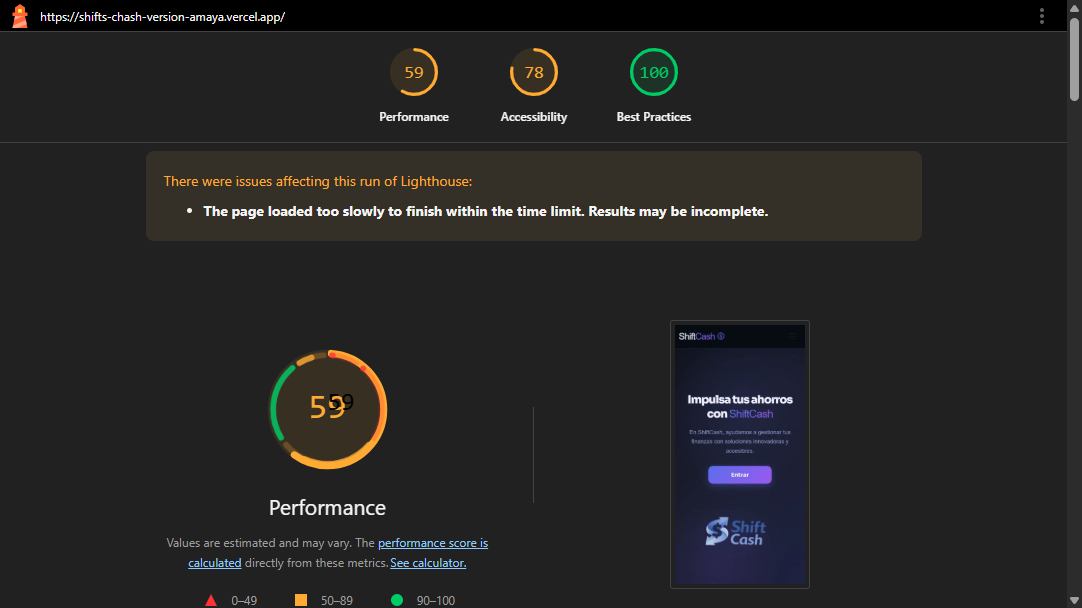
\includegraphics[width=0.49\linewidth]{../evidencias/lighthouse/vercel.png}\hfill
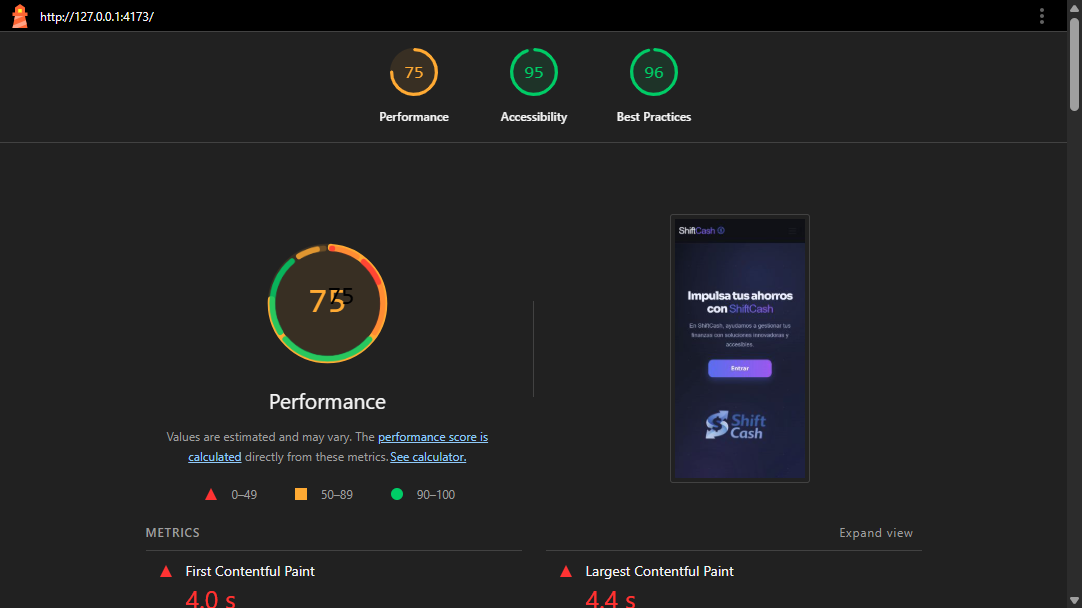
\includegraphics[width=0.49\linewidth]{../evidencias/lighthouse/local.png}
\figurenote{Fuente: elaboración propia con Lighthouse 12.8.2.}
\end{figure}

\paragraph{Mejoras aplicadas.} La portada descargaba todo el código del dashboard (incluido Recharts) y un logotipo PNG de 297 kB y 1500 × 1000 px. Cargamos el dashboard con \codigo{React.lazy} y reemplazamos el logotipo por un WebP de 29 kB a 750 × 500 px. El LCP en perfil de escritorio cumple el objetivo; en perfil móvil bajó de 6,9 a 4,4 s, todavía por encima de 2,5 s, porque el contenido se dibuja después de cargar las hojas de estilo y fuentes externas (Bootstrap y Google Fonts) y de ejecutar React.

\subsection{Compatibilidad}

\metricas{Métricas de compatibilidad}{tab:me-compatibilidad}{%
Interoperabilidad & Routers con contrato REST/JSON publicado en OpenAPI & — & 1,00 & 6/6 = 1,00 & 6/6 = 1,00 \\
Interoperabilidad & Integraciones externas operativas: $\frac{\text{operativas}}{\text{declaradas en la interfaz}}$ & — & 1,00 & 1/2 = 0,50 (Facebook sin implementar) & 1/2 = 0,50 \\
Coexistencia & Servicios que se despliegan y escalan por separado & — & 1,00 & 3/3 (Vercel, Render, Supabase) & 3/3 \\
}{Herramientas: \codigo{/openapi.json} de FastAPI e inspección de la interfaz. Fuente: elaboración propia.}

\subsection{Usabilidad}

\metricas{Métricas de usabilidad}{tab:me-usabilidad}{%
Accesibilidad & Puntaje de accesibilidad de Lighthouse (móvil) & RNF14 & $\geq 90$ & 78 & 95 \\
Accesibilidad & Campos con etiqueta asociada en el formulario de contacto & RNF14 & 1,00 & 0/3 = 0,00 & 3/3 = 1,00 \\
Accesibilidad & Botones con nombre accesible en la portada & RNF14 & 1,00 & Menú sin nombre & 1,00 (\codigo{aria-label}) \\
Operabilidad & Mediana del tiempo para registrar un gasto (PU-06) & RNF07 & $\leq 60$ s & No medido & \resPUMediana{} s \\
Operabilidad & Tasa de éxito al primer intento (PU-06) & RNF07 & $\geq 0{,}90$ & No medido & \resPUExito \\
Protección frente a errores & Errores de validación de la API mostrados como texto legible & RNF05 & 1,00 & 0 (un 422 rompía el formulario, D-13) & 1,00 \\
}{Lighthouse marca aún el contraste de un texto de la portada (\codigo{text-primary}). Fuente: elaboración propia.}

\subsection{Fiabilidad}

\metricas{Métricas de fiabilidad}{tab:me-fiabilidad}{%
Madurez & Pruebas automatizadas sin fallos: $\frac{\text{aprobadas}}{\text{ejecutadas}}$ & — & 1,00 & 48/49 = 0,98 & 95/95 = 1,00 \\
Disponibilidad & Tiempo operativo del frontend en la ventana de prueba & RNF10 & $\geq 0{,}99$ & 1,00 & 1,00 \\
Disponibilidad & Tiempo operativo de la API en la ventana de prueba & RNF10 & $\geq 0{,}99$ & 0,00 (más de 7 min sin respuesta) & \resDisponibilidadApi \\
Tolerancia a fallos & Entradas inválidas respondidas con 4xx: $\frac{\text{4xx}}{\text{entradas inválidas probadas}}$ & RNF05 & 1,00 & 4/6 = 0,67 & 5/5 = 1,00 (la meta sin fecha final ahora es una entrada válida) \\
Recuperabilidad & Recurrentes que no se duplican al reejecutar el programador & — & 1,00 & No ejecutado & 1,00 (PI-08) \\
}{Herramientas: pytest, Cypress y observación del servicio. Fuente: elaboración propia.}

\subsection{Seguridad}

\metricas{Métricas de seguridad}{tab:me-seguridad}{%
Autenticidad & Endpoints de datos que exigen JWT: $\frac{\text{protegidos}}{\text{de datos}}$ & RNF02 & 1,00 & 26/26 = 1,00 & 26/26 = 1,00 \\
Confidencialidad & Contraseñas guardadas con hash: $\frac{\text{con hash}}{\text{guardadas}}$ & RNF01 & 1,00 & 1,00 & 1,00 \\
Confidencialidad & Credenciales escritas en el código & RNF13 & 0 & 2 (D-06) & 0 \\
Confidencialidad & Registros ajenos visibles o modificables & RNF12 & 0 & 0 (estático) & 0 (ejecutado) \\
Integridad & Campos críticos validados en el servidor (F1–F3): $\frac{\text{validados}}{14}$ & RNF05 & 1,00 & 9/14 = 0,64 & 14/14 = 1,00 \\
Integridad & Orígenes no autorizados que reciben cabeceras CORS & RNF03 & 0 & 0 (estático) & 0 (ejecutado) \\
Resistencia & Alertas de ZAP de riesgo alto / medio & RNF13 & 0 / 0 & 0 / 3 & \resZapResumen \\
}{Los 14 campos críticos son: en transacciones, monto mínimo, monto máximo, tipo, categoría y frecuencia; en presupuestos, monto, período, mes, año y fechas del período único; en metas, nombre, objetivo, fecha final y orden de fechas. La frecuencia se validó al corregir D-14. Fuente: elaboración propia.}

\subsection{Mantenibilidad}

\metricas{Métricas de mantenibilidad}{tab:me-mantenibilidad}{%
Analizabilidad & Funciones con $V(G) \leq 10$: $\frac{A}{B}$ & RNF09 & 1,00 & 55/58 = 0,95 & 92/92 = 1,00 \\
Analizabilidad & Densidad de comentarios del Python & — & — & 93/1\,657 = 0,056 & 57/1\,478 = 0,039 \\
Modularidad & CBO medio de los routers & — & $\leq 6$ & 4,0 & 4,7 \\
Reusabilidad & Construcciones de respuesta duplicadas & — & 0 & 6 & 0 \\
Modificabilidad & Elementos de código muerto & — & 0 & 3 & 0 \\
Capacidad de prueba & Cobertura de líneas del backend & RNF09 & $\geq 0{,}80$ & 0,00 & 0,95 \\
}{Herramientas: \codigo{metricas.py}, pytest-cov y SonarQube (antes: mantenibilidad A, 249 incidencias; después: \resSonar). Fuente: elaboración propia.}

\subsection{Portabilidad}

\metricas{Métricas de portabilidad}{tab:me-portabilidad}{%
Adaptabilidad & Resoluciones sin desbordamiento: $\frac{\text{correctas}}{\text{probadas}}$ & RNF06 & 1,00 & 2/2 & 2/2 \\
Adaptabilidad & Navegadores verificados: $\frac{\text{correctos}}{4}$ (Chrome, Firefox, Edge, Safari) & RNF06 & 1,00 & 2/4 = 0,50 & \resNavegadores \\
Instalabilidad & Pasos de instalación documentados: $\frac{\text{en el README}}{\text{necesarios}}$ & — & 1,00 & 3/6 = 0,50 & 6/6 = 1,00 \\
}{Los seis pasos son: clonar, instalar y configurar el backend (\codigo{.env}), levantar la API, instalar el frontend, configurar \codigo{.env.local} y levantar el frontend. Fuente: elaboración propia.}

\section{Conclusiones de la medición}

\paragraph{Calidad interna.} La refactorización redujo la complejidad sin aumentar el tamaño: el código de lógica bajó de 6\,228 a 6\,125 líneas, ninguna función supera $V(G) = 10$ (antes, tres), la complejidad media bajó de 3,4 a 2,2 y las rutas pasaron de WMC 50 y 37 a 7 y 5. El acoplamiento y la herencia siguen en los rangos comunes del catálogo de \textcite{filo2015}. El único valor poco común es el WMC de \codigo{saving_service} (39), que proponemos dividir.

\paragraph{Calidad externa.} Mejoraron la corrección funcional (0,90 → 1,00), la integridad de las entradas (0,64 → 1,00), la tolerancia a fallos (0,67 → 1,00), la accesibilidad (78 → 95), la instalabilidad (0,50 → 1,00) y la capacidad de prueba (cobertura de 0 a 95\,\%). Siguen por debajo del objetivo el LCP en perfil móvil (4,4 s frente a 2,5 s) y la verificación en Edge y Safari, y faltan por medir la disponibilidad de la API en Render, la tarea PU-06 y los nuevos escaneos de ZAP y SonarQube.
